\section{Graph}
\markright{Graph}

The Zener diode characteristic has been plotted separately for the forward and reverse bias regions because the two regions operate over very different voltage and current ranges. This allows the knee of the forward characteristic and the breakdown region of the reverse characteristic to be observed more clearly.

\begin{figure}[H]
  \centering
  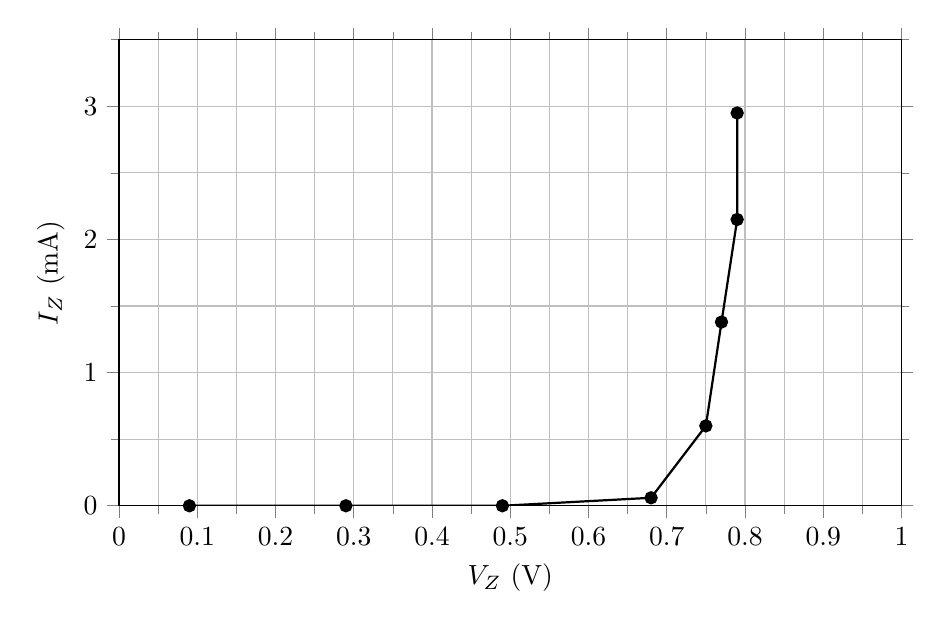
\begin{tikzpicture}
    \begin{axis}[
        width=0.95\textwidth,
        height=7.5cm,
        xlabel={$V_Z$ (V)},
        ylabel={$I_Z$ (mA)},
        xmin=0,
        xmax=1.0,
        ymin=0,
        ymax=3.5,
        grid=both,
        major grid style={gray!50},
        minor tick num=1,
        tick align=outside,
        enlargelimits=false
      ]
      \addplot[black, mark=*, thick] coordinates {
          (0.09,0.00)
          (0.29,0.00)
          (0.49,0.00)
          (0.68,0.06)
          (0.75,0.60)
          (0.77,1.38)
          (0.79,2.15)
          (0.79,2.95)
        };
    \end{axis}
  \end{tikzpicture}
  \caption{Forward-bias characteristic curve of the Zener diode.}
  \label{fig:lab06_forward_curve}
\end{figure}

\begin{figure}[H]
  \centering
  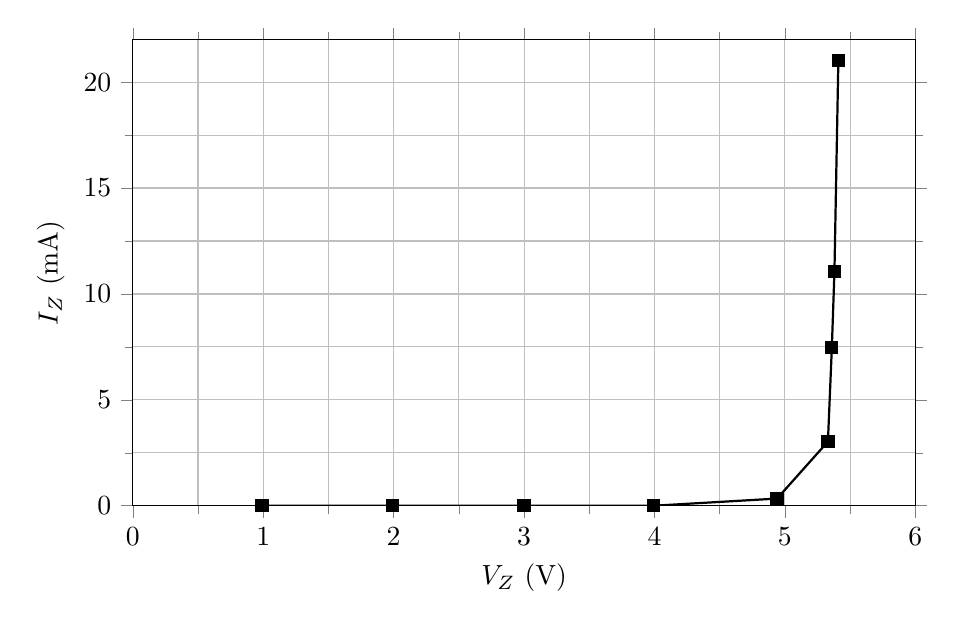
\begin{tikzpicture}
    \begin{axis}[
        width=0.95\textwidth,
        height=7.5cm,
        xlabel={$V_Z$ (V)},
        ylabel={$I_Z$ (mA)},
        xmin=0,
        xmax=6,
        ymin=0,
        ymax=22,
        grid=both,
        major grid style={gray!50},
        minor tick num=1,
        tick align=outside,
        enlargelimits=false
      ]
      \addplot[black, mark=square*, thick] coordinates {
          (0.99,0.00)
          (1.99,0.00)
          (3.00,0.00)
          (3.99,0.00)
          (4.94,0.34)
          (5.33,3.03)
          (5.36,7.46)
          (5.38,11.06)
          (5.41,21.01)
        };
    \end{axis}
  \end{tikzpicture}
  \caption{Reverse-bias characteristic curve of the Zener diode in breakdown region.}
  \label{fig:lab06_reverse_curve}
\end{figure}

From the two graphs, it is observed that the forward current rises sharply after a small forward voltage, while in reverse bias the voltage stays nearly constant at about $5.4\,\text{V}$ once the breakdown region is reached. This behavior confirms the Zener diode's use as a voltage regulator.
